\section{Quantum Particle in Fermi System}
\subsection{Propagator method in many-body systems}
In this chapter we will start with non-interacting Fermi-system problem. This is really a fake many-body problem,since as the problem is actually only a one-body problem. By doing this trivial problem, we will describe Fermi system very simply in terms of a few particles above the Fermi level, and a few removed particles, or "holes" below. Second, it allows us to introduce the language of the many-body problem,"\bluep{occupation number formalism}", or "\bluep{second quantization}". Finally, it shows us how to extend the definition of the propagator to the case where $t_2<t_1$. In this case, \textbf{the Green's function turns out to describe the propagation of removed particles, or "holes", which are represented diagrammatically by a downward-going arrow.}

By introducing a tree-level two-body interaction 
\begin{center}
\tikzset{every picture/.style={line width=0.75pt}} %set default line width to 0.75pt        

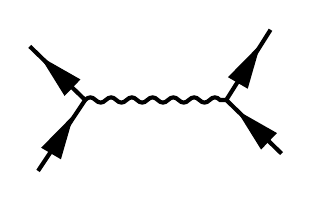
\begin{tikzpicture}[x=0.75pt,y=0.75pt,yscale=-1,xscale=1]
%uncomment if require: \path (0,705); %set diagram left start at 0, and has height of 705

%Straight Lines [id:da613823184290475] 
\draw [line width=1.5]    (491.42,548.13) .. controls (493.09,546.46) and (494.75,546.46) .. (496.42,548.13) .. controls (498.09,549.8) and (499.75,549.8) .. (501.42,548.13) .. controls (503.09,546.46) and (504.75,546.46) .. (506.42,548.13) .. controls (508.09,549.8) and (509.75,549.8) .. (511.42,548.13) .. controls (513.09,546.46) and (514.75,546.46) .. (516.42,548.13) .. controls (518.09,549.8) and (519.75,549.8) .. (521.42,548.13) .. controls (523.09,546.46) and (524.75,546.46) .. (526.42,548.13) .. controls (528.09,549.8) and (529.75,549.8) .. (531.42,548.13) .. controls (533.09,546.46) and (534.75,546.46) .. (536.42,548.13) .. controls (538.09,549.8) and (539.75,549.8) .. (541.42,548.13) .. controls (543.09,546.46) and (544.75,546.46) .. (546.42,548.13) .. controls (548.09,549.8) and (549.75,549.8) .. (551.42,548.13) .. controls (553.09,546.46) and (554.75,546.46) .. (556.42,548.13) -- (559.42,548.13) -- (559.42,548.13) ;
%Straight Lines [id:da6353755682299548] 
\draw [line width=1.5]    (464.75,522.3) -- (491.42,548.13) ;
%Straight Lines [id:da6254606220772768] 
\draw [line width=1.5]    (559.42,548.13) -- (586.08,573.97) ;
%Straight Lines [id:da5480869883300985] 
\draw [line width=1.5]    (491.42,548.13) -- (468.75,582.3) ;
%Straight Lines [id:da49445752084181116] 
\draw [line width=1.5]    (580.75,514.3) -- (559.42,548.13) ;
%Shape: Triangle [id:dp022384072825595847] 
\draw  [fill={rgb, 255:red, 0; green, 0; blue, 0 }  ,fill opacity=1 ] (471.18,528.57) -- (488.37,538.35) -- (481.61,545.37) -- cycle ;
%Shape: Triangle [id:dp5669679661948073] 
\draw  [fill={rgb, 255:red, 0; green, 0; blue, 0 }  ,fill opacity=1 ] (565.84,554.41) -- (583.04,564.18) -- (576.28,571.21) -- cycle ;
%Shape: Triangle [id:dp23872151900315752] 
\draw  [fill={rgb, 255:red, 0; green, 0; blue, 0 }  ,fill opacity=1 ] (574.92,522.94) -- (569.46,541.95) -- (561.04,537.03) -- cycle ;
%Shape: Triangle [id:dp5504301680867448] 
\draw  [fill={rgb, 255:red, 0; green, 0; blue, 0 }  ,fill opacity=1 ] (484.92,556.94) -- (479.46,575.95) -- (471.04,571.03) -- cycle ;




\end{tikzpicture}
\end{center}
we again can represent the propagator for this case as an infinite series of diagrams, which may be evaluated approximately by partial summation.

\bluep{The Hartree and Hartree-Fock are the crudest of the approximations and yield quasi particles with infinite lifetimes. The RPA yields the energy and lifetime of quasi particles in a high-density electron gas, while the ladder approxiamation is good for low-density systems like nuclear matter. Only the Hartree and Hartree-Fock will be discussed in this chapter.}
\begin{table}[H]
        \centering
        \caption{Some important partial sum approx.}
\begin{tabular}{|p{0.45\textwidth}|p{0.33\textwidth}|}
\hline 
 \begin{center}
{\fontfamily{helvet}\selectfont Types of diagrams summed over}
\end{center}
 & \begin{center}
{\fontfamily{helvet}\selectfont Name of approximation}
\end{center}
 \\
\hline 
 \begin{center}
{\fontfamily{helvet}\selectfont Bubbles}
\end{center}
 & \begin{center}
{\fontfamily{helvet}\selectfont Hartree}
\end{center}
 \\
\hline 
 \begin{center}
{\fontfamily{helvet}\selectfont Bubbles and open oysters}
\end{center}
 & \begin{center}
{\fontfamily{helvet}\selectfont Hartree-Fock}
\end{center}
 \\
\hline 
 \begin{center}
{\fontfamily{helvet}\selectfont Rings}
\end{center}
 & \begin{center}
{\fontfamily{helvet}\selectfont Random phase approx(RPA)}
\end{center}
 \\
\hline 
 \begin{center}
{\fontfamily{helvet}\selectfont Ladders}
\end{center}
 & \begin{center}
{\fontfamily{helvet}\selectfont Ladder approximation}
\end{center}
 \\
 \hline
\end{tabular}
        \end{table}
\subsection{Non-interacting Fermi system in external potential: particle- hole picture}
We first introduce the particle-hole nomenclature for describing Fermi systems. Suppose we have a single particle in a potential $U(\mathbf{r})$, with energy eigenstates $\phi_k(\mathbf{r})$. The energy levels may be represented as in Fig.\ref{fig:non-interacting-fermi},where for simplicity the system is non-degenerate.
\begin{figure}[H]
    \centering
    \includegraphics[scale=0.6]{screenshots/particle-hole.PNG}
    \caption{Non-interacting Fermi System}
    \label{fig:non-interacting-fermi}
\end{figure}
In the case where $U(\mathbf{r})=0$, the particles are free and $\mathbf{k}$ in \ref{fig:non-interacting-fermi}(a) are momentum, or wavenumber. The ground state of the single particle has energy $\epsilon_F$. If we now put N particles into the system, by Pauli principle the energy levels will be filled from the bottom as shown in \ref{fig:non-interacting-fermi}(a) for $N=5$. The highest filled energy level is the \textit{\textbf{Fermi level}},$\epsilon_F$. In ground state, the free particles fill a sphere in $\mathbf{k}-$space having radius $k_F=\sqrt{2m\epsilon_F}$,where $k_F$ is called the \textbf{Fermi momentum}. The filled sphere is called Fermi sea. The surface of this sphere is \textbf{Fermi surface}.

In Fig \ref{fig:non-interacting-fermi}(b) the excited states of the system are formed by removing a particle from a state below $\epsilon_F$ to a state above. The empty state here is called "hole". In "\bluep{particle-hole description}" we can omit the filled Fermi sea and only focus on excited particle and holes, yielding \ref{fig:non-interacting-fermi}(c) and (d). \textbf{\redp{Since a hole in state $\phi_k$ is actually removal of a particle from the system, the hole represents energy $\epsilon_k$ removed. Hence the hole energy is}}
\begin{equation}\epsilon_{k}^{\text {hole }}=-\epsilon_{k}\end{equation}
The time-dependent wave function is thus
\begin{equation}\psi_{k}(t)^{\text {hole }}=\phi_{k} e^{-i\left(-\epsilon_{k}\right) t}, \quad \epsilon_{k}<\epsilon_{F}\end{equation}
\subsection{A primer of second quantization formalism}
The total wave function for the ground and excited states of a system of non-interacting particles is the Slater determinant:
\begin{equation}\Phi_{k_{1}, \ldots, k_{N}}\left(\mathbf{r}_{1}, \ldots, \mathbf{r}_{N}\right)=\frac{1}{\sqrt{(N !)}}\left|\begin{array}{cc}
\phi_{k_{1}}\left(\mathbf{r}_{1}\right) \ldots \phi_{k_{1}}\left(\mathbf{r}_{N}\right) \\
\vdots & \vdots \\
\phi_{k_{N}}\left(\mathbf{r}_{1}\right) \ldots \phi_{k_{N}}\left(\mathbf{r}_{N}\right)
\end{array}\right|
\label{slater-determinant}
\end{equation}
\textbf{If the particles are allowed to interact with each other or external potential,} then the exact wave function of the system is a linear combination of \ref{slater-determinant}:
\begin{equation}\Psi\left(\mathbf{r}_{1}, \ldots, \mathbf{r}_{N}\right)=\sum_{k_{1}, \ldots, k_{N}} A_{k_{1}, \ldots, k_{N}} \Phi_{k_{1}, \ldots, k_{N}}\left(\mathbf{r}_{1}, \ldots, \mathbf{r}_{N}\right)\end{equation}
That is, the $\Phi_{k_1,k_2,\ldots}$ for the non-interacting system are the basis states used to describe the interacting system. Noting that all particles are indistinguishable, the essential information in \ref{slater-determinant} is just how many particles in each state, $n$. For short, we shall represent this as
\begin{equation}
    \Phi_{k_1,k_2,\ldots}=\left|n_{p_1},n_{p_2},\ldots\right\rangle
\label{linear-comb-occ-vec}
\end{equation}
meaning:$n_{p_{1}}$ particles in state $\phi_{p_{1}}, n_{p_{2}}$ in $\phi_{p_{3}},$ etc., where $n=0$ or 1 by Pauli principle. This notation is called "\redp{occupation number notation}". It is important to note that just as the original Slater determinant form a complete orthogonal set of basis functions, so do the states in occupation number notation and we have
\begin{equation}\left\langle n_{1}^{\prime}, \ldots n_{i}^{\prime} \ldots | n_{1}, \ldots, n_{i} \ldots\right\rangle=\delta_{n_1^{\prime}n_1}\ldots\delta_{n_i^{\prime}n_i}\ldots
\end{equation}
The wave function for interacting system is now becoming:
\begin{equation}\Psi=\sum_{n_{1}, \ldots, n_{i}, \ldots} A_{n_{1}, \ldots, n_{i}, \ldots}\left|n_{1}, \ldots, n_{i}, \ldots\right\rangle\end{equation}
In the particle-hole notation, it is necessary to introduce hole creation and destruction operators, $b_1^{\dagger}, b_{1}$, and similarly particle operators $a_1^{\dagger}, a_{1},$ as follows:
if $k_{i}<k_{F},$ then $c_{i}$ destroys a particle under the Fermi level, thus creating a hole. Hence
\begin{equation}\begin{aligned}
\text { for } k_{l}>k_{F}, & c_{l}=a_{l} \\
k_{l}<k_{F}, & c_{l}=b^{\dagger}_l
\end{aligned}\end{equation}
and
\begin{equation}\begin{aligned}
\text { for } k_{l}>k_{F}, & c_{l}^{\dagger}=a_{l}^{\dagger} \\
k_{l}<k_{F}, & c_{l}^{\dagger}=b_{l}
\end{aligned}\end{equation}
Simple examples of how the particle-hole operators work are:
$$a_{i}^{\dagger}|0\rangle=\left|1_i^{p}\right\rangle, \quad a_{i}\left|1_l^{p}\right\rangle=\delta_{il}|0\rangle, \quad b_{j}^{\dagger} a_{i}^{\dagger}\left|1_{m}^{\rho}\right\rangle=\left|1_{m}^{p}, 1_i^{p}, 1_j^{h}\right\rangle$$
where the superscripts represent "particle" and "hole", respectively. \redp{The operator in the occupation number formalism, $\mathcal{O}^{occ}$ is:}
\begin{equation}\mathcal{O}^{occ}=\sum_{m n} \mathcal{O}_{m n} c_{m}^{\dagger} c_{n}\end{equation}
where
\begin{equation}\begin{array}{l}
c_{l}=\theta_{k_{l}-k_{F}} a_{l}+\theta_{k_{F-k_{l}}} b_{l}^{\dagger} \\
c_{l}^{\dagger}=\theta_{k_{1}-k_{F}} a_{l}^{\dagger}+\theta_{k_{F}-k_{l}} b_{l}
\end{array}\end{equation}
and $\theta_{x}=1$ for $x>0 ; \quad \theta_{x}=0$ for $x<0$.

The Hamiltonian for an arbitrary system may be expressed in occupation number or particle-hole formalism. Suppose the system Hamiltonian in old Neanderthal notation describes a system in an external perturbing potential:
\begin{equation}H_{\text {Neand. }}=\underbrace{\sum_{i}\left[\frac{p_{1}^{2}}{2 m}+U\left(\mathbf{r}_{i}\right)\right]}_{H_{0}}+\underbrace{\sum_{i} V\left(\mathbf{r}_{i}\right)}_{H_{1}(\text { perturbation })}\end{equation}
The single-particle states $\phi_k$ satisfy:
\begin{equation}\left[\frac{p^{2}}{2 m}+U(\mathbf{r})\right] \phi_{k}=\epsilon_{k} \phi_{k}\end{equation}
Then it is found that
\begin{equation}H_{0}=\sum_{k} \epsilon_{k} c^{\dagger}_{k} c_{k}=\sum_{k>k_{F}} \epsilon_{k} a_{k}^{\dagger} a_{k}+\sum_{k<k_{F}} \epsilon_{k} b_{k} b^{\dagger}_{k}
\label{H0-Nead}
\end{equation}
\begin{equation}\begin{aligned}
H_{1}=& \sum_{m, n>k_{F}} V_{m n} a_{m}^{\dagger} a_{n}+\sum_{m>k_{F},n<k_F} V_{m n} a_{m}^{\dagger} b_{n}^{\dagger}+\sum_{m<k_{F}, n>k_{F}} V_{m n} b_{m} a_{n}+\\
&+\sum_{m, n<k_{F}} V_{m n} b_{m} b_{n}^{\dagger}
\end{aligned}
\label{H1}
\end{equation}
For a system of mutually interacting particles with a Hamiltonian
\begin{equation}H_{\mathrm{old}}=\underbrace{\sum_{l} \frac{p_{l}^{2}}{2 m}}_{H_{0}}+\frac{1}{2} \underbrace{\sum_{i, J} V\left(\mathbf{r}_{i}-\mathbf{r}_{j}\right)}_{H_{1}(\text { perturbation })}
\label{mutual-interact-hamiltonian}
\end{equation}
We also find that
\begin{equation}H_{0}=\sum_{k>k_{F}} \epsilon_{k} a_{k}^{\dagger} a_{k}+\sum_{k<k_{F}} \epsilon_{k} b_{k} b^{\dagger}_{k}\quad\epsilon_k=k^2/2m\end{equation}
\begin{equation}\begin{aligned}
H_{1}&=\frac{1}{2} \sum_{k, l, m, n>k_{F}} V_{k l m n} a_{l}^{\dagger} a_{k}^{\dagger} a_{m} a_{n}+\sum_{k, l, m>k_{F};n<k_F} V_{k l m n} a_{l}^{\dagger} a^{\dagger}_{k} a_{m} b_{n}^{\dagger}+\\
&+\cdots+\frac{1}{2} \sum_{k, l, m, n<k_{r}} V_{k l m n} b_{l} b_{k} b_{m}^{\dagger} b_{n}^{\dagger}
\end{aligned}
\label{mutual-interact-H1}
\end{equation}
We will define $V_{klmn}$ later. It should be carefully remembered that \textbf{\bluep{in the case of interacting system, the wave functions  are given by the linear combination of \ref{linear-comb-occ-vec}.}}

\subsection{Propagator for non-interacting Fermi system in external perturbing potential}
To treat the general situation of "holes", we extend the definition of propagator to times $t_2<t_1$. This leads us to the definition:
\begin{imp}
\begin{equation}
    iG(k_2,k_1,t_2-t_1)_{t_2<t_1}\equiv i G^{-}\left(k_{2}, k_{1}, t_{2}-t_{1}\right)
\end{equation}
which is $-1\times$probability amplitude that if at time $t_{2}$ we remove a particle in state $\phi_{k_{2}}$ from (i.e., if we add a hole in $\phi_{k_{2}}$ to) the interacting system in its ground state, then at time $t_{1}$ the system will be in its ground state with a particle removed from (i.e., an added hole in $) \phi_{k_{1}}$.\bluep{ The factor of (-1) here compared with $iG^+$ comes because we have fermions. Note that $G^-$ is called an "advanced" propagator or Green's function.}
\end{imp}
\redp{for $\left.t_{2}>t_{1} \text { (but not for } t_{2}=t_{1} !\right), G^{-}$ is defined so that}
\begin{equation}i G^{-}\left(k_{2}, k_{1}, t_{2}-t_{1}\right)_{t_{2}>r_{1}}=0\end{equation}

In the case of a free hole, we have
\begin{equation}G_{0}^{-}\left(k, t_{2}-t_{1}\right)=\left\{\begin{array}{l}
i \theta_{t_{1}-t_{2}} e^{-i \epsilon_{k}\left(t_{2}-t_{1}\right)}\quad t_2\neq t1,\epsilon_k<\epsilon_F \\
i, \quad \text { for } t_{2}=t_{1}
\end{array}\right.
\label{Gminus-t-space}
\end{equation}
with Fourier transform
\begin{equation}G_{0}^{-}(k, \omega)=\frac{1}{\omega-\epsilon_{k}-i \delta}, \quad \epsilon_{k}<\epsilon_{F}
\label{Gminus-k-space}
\end{equation}
The interaction amplitude, $V_{kl}$, merits some discussion. It is given by 
\begin{equation}V_{k l}=\int d^{3} \mathbf{r} \phi_{k}^{*}(\mathbf{r}) V(\mathbf{r}, \mathbf{p}) \phi_{l}(\mathbf{r})
\label{Vkl}
\end{equation}
There are four possibilities of $V_{kl}$ shown in the table below. They mean:(a) scattering of a particle in particle-hole formalism from state $\phi_{l}$ to $\phi_{k},$ (b) the potential scatters a particle out of state $\phi_{l},$ where $\epsilon_{l}<\epsilon_{F},$ into state $\phi_{k}, \epsilon_{k}>\epsilon_{F},$ thus simultaneously creating a particle in $\phi_{k}$ and a hole in $\phi_{l},(c),$ etc. \redp{Note that these four possibilities correspond to the four interaction terms in the particle-hole Hamiltonian for this case (\ref{mutual-interact-hamiltonian})}.
\begin{figure}[H]
    \centering
\tikzset{every picture/.style={line width=0.75pt}} %set default line width to 0.75pt        
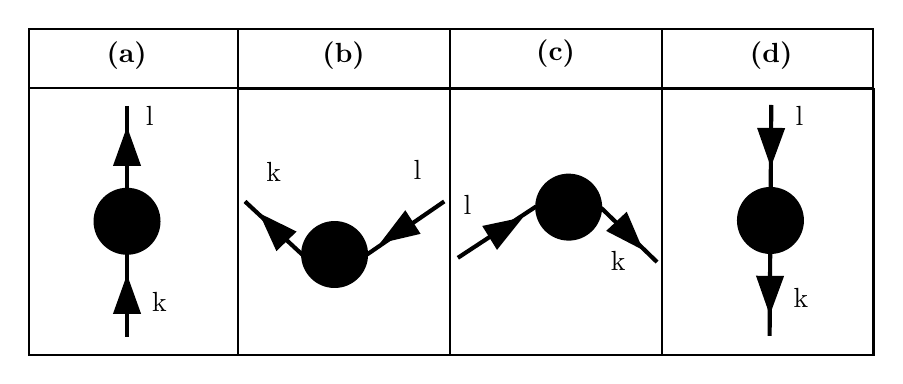
\begin{tikzpicture}[x=0.75pt,y=0.75pt,yscale=-1,xscale=1]
%uncomment if require: \path (0,244); %set diagram left start at 0, and has height of 244

%Shape: Circle [id:dp7355643708429443] 
\draw  [fill={rgb, 255:red, 0; green, 0; blue, 0 }  ,fill opacity=1 ] (147.73,133.97) .. controls (147.73,125.33) and (154.73,118.33) .. (163.37,118.33) .. controls (172,118.33) and (179,125.33) .. (179,133.97) .. controls (179,142.6) and (172,149.6) .. (163.37,149.6) .. controls (154.73,149.6) and (147.73,142.6) .. (147.73,133.97) -- cycle ;
%Straight Lines [id:da3859042750603179] 
\draw [line width=1.5]    (163.37,149.6) -- (163.37,189.6) ;
%Straight Lines [id:da7654556741518936] 
\draw [line width=1.5]    (163.37,78.33) -- (163.37,118.33) ;
%Shape: Triangle [id:dp19291169740752956] 
\draw  [fill={rgb, 255:red, 0; green, 0; blue, 0 }  ,fill opacity=1 ] (163.37,89.87) -- (169.43,106.79) -- (157.3,106.79) -- cycle ;
%Shape: Triangle [id:dp3466064725515261] 
\draw  [fill={rgb, 255:red, 0; green, 0; blue, 0 }  ,fill opacity=1 ] (163.37,161.14) -- (169.43,178.06) -- (157.3,178.06) -- cycle ;
%Shape: Circle [id:dp605096323889595] 
\draw  [fill={rgb, 255:red, 0; green, 0; blue, 0 }  ,fill opacity=1 ] (247.73,149.97) .. controls (247.73,141.33) and (254.73,134.33) .. (263.37,134.33) .. controls (272,134.33) and (279,141.33) .. (279,149.97) .. controls (279,158.6) and (272,165.6) .. (263.37,165.6) .. controls (254.73,165.6) and (247.73,158.6) .. (247.73,149.97) -- cycle ;
%Straight Lines [id:da59504555135735] 
\draw [line width=1.5]    (279,149.97) -- (316.2,124.4) ;
%Straight Lines [id:da3713869779792379] 
\draw [line width=1.5]    (220.2,124.4) -- (247.73,149.97) ;
%Shape: Triangle [id:dp6549052988211023] 
\draw  [fill={rgb, 255:red, 0; green, 0; blue, 0 }  ,fill opacity=1 ] (228.08,131.11) -- (244.21,139.04) -- (235.5,147.48) -- cycle ;
%Shape: Triangle [id:dp6944058778949381] 
\draw  [fill={rgb, 255:red, 0; green, 0; blue, 0 }  ,fill opacity=1 ] (286.5,143.78) -- (297.41,129.5) -- (304,139.68) -- cycle ;
%Shape: Circle [id:dp5744676253853855] 
\draw  [fill={rgb, 255:red, 0; green, 0; blue, 0 }  ,fill opacity=1 ] (391.77,127.47) .. controls (391.58,136.11) and (384.44,142.95) .. (375.8,142.77) .. controls (367.17,142.58) and (360.32,135.43) .. (360.51,126.8) .. controls (360.69,118.17) and (367.84,111.32) .. (376.47,111.51) .. controls (385.11,111.69) and (391.95,118.84) .. (391.77,127.47) -- cycle ;
%Straight Lines [id:da9080029217596884] 
\draw [line width=1.5]    (360.51,126.8) -- (322.77,151.56) ;
%Straight Lines [id:da5417814826950174] 
\draw [line width=1.5]    (418.75,153.63) -- (391.77,127.47) ;
%Shape: Triangle [id:dp21341953231164135] 
\draw  [fill={rgb, 255:red, 0; green, 0; blue, 0 }  ,fill opacity=1 ] (411.01,146.75) -- (395.06,138.48) -- (403.95,130.22) -- cycle ;
%Shape: Triangle [id:dp18680249773366642] 
\draw  [fill={rgb, 255:red, 0; green, 0; blue, 0 }  ,fill opacity=1 ] (352.88,132.83) -- (341.67,146.87) -- (335.3,136.55) -- cycle ;
%Shape: Circle [id:dp23848631002762677] 
\draw  [fill={rgb, 255:red, 0; green, 0; blue, 0 }  ,fill opacity=1 ] (489,133.68) .. controls (488.94,142.32) and (481.89,149.26) .. (473.25,149.2) .. controls (464.62,149.14) and (457.67,142.09) .. (457.73,133.45) .. controls (457.8,124.82) and (464.85,117.87) .. (473.48,117.93) .. controls (482.12,118) and (489.06,125.05) .. (489,133.68) -- cycle ;
%Straight Lines [id:da48621128625100807] 
\draw [line width=1.5]    (473.48,117.93) -- (473.77,77.93) ;
%Straight Lines [id:da07279871641659819] 
\draw [line width=1.5]    (472.96,189.2) -- (473.25,149.2) ;
%Shape: Triangle [id:dp6526600818062779] 
\draw  [fill={rgb, 255:red, 0; green, 0; blue, 0 }  ,fill opacity=1 ] (473.04,177.66) -- (467.1,160.7) -- (479.23,160.79) -- cycle ;
%Shape: Triangle [id:dp49414286713798516] 
\draw  [fill={rgb, 255:red, 0; green, 0; blue, 0 }  ,fill opacity=1 ] (473.57,106.39) -- (467.62,89.43) -- (479.76,89.52) -- cycle ;
%Shape: Rectangle [id:dp23062556048857352] 
\draw   (116,69.87) -- (217,69.87) -- (217,198.18) -- (116,198.18) -- cycle ;
%Shape: Rectangle [id:dp4116028056497356] 
\draw   (217,70.18) -- (319,70.18) -- (319,198.18) -- (217,198.18) -- cycle ;
%Shape: Rectangle [id:dp7757074524824593] 
\draw   (319,70.18) -- (421,70.18) -- (421,198.18) -- (319,198.18) -- cycle ;
%Shape: Rectangle [id:dp537554675418955] 
\draw   (421,70.18) -- (523,70.18) -- (523,198.18) -- (421,198.18) -- cycle ;
%Shape: Rectangle [id:dp8001518431361148] 
\draw   (116,41.18) -- (217,41.18) -- (217,69.87) -- (116,69.87) -- cycle ;
%Shape: Rectangle [id:dp6414334269575042] 
\draw   (217,41.18) -- (318.95,41.18) -- (318.95,69.87) -- (217,69.87) -- cycle ;
%Shape: Rectangle [id:dp059392457734880444] 
\draw   (318.95,41.18) -- (420.9,41.18) -- (420.9,69.87) -- (318.95,69.87) -- cycle ;
%Shape: Rectangle [id:dp2648624460179885] 
\draw   (420.9,41.18) -- (522.85,41.18) -- (522.85,69.87) -- (420.9,69.87) -- cycle ;

% Text Node
\draw (152,45.85) node [anchor=north west][inner sep=0.75pt]   [align=left] {\textbf{(a)}};
% Text Node
\draw (256,45.85) node [anchor=north west][inner sep=0.75pt]   [align=left] {\textbf{(b)}};
% Text Node
\draw (359,44.85) node [anchor=north west][inner sep=0.75pt]   [align=left] {\textbf{(c)}};
% Text Node
\draw (462,45.85) node [anchor=north west][inner sep=0.75pt]   [align=left] {\textbf{(d)}};
% Text Node
\draw (174,166.85) node [anchor=north west][inner sep=0.75pt]   [align=left] {k};
% Text Node
\draw (171,76.85) node [anchor=north west][inner sep=0.75pt]   [align=left] {l};
% Text Node
\draw (300,102.85) node [anchor=north west][inner sep=0.75pt]   [align=left] {l};
% Text Node
\draw (324,119.85) node [anchor=north west][inner sep=0.75pt]   [align=left] {l};
% Text Node
\draw (484,76.85) node [anchor=north west][inner sep=0.75pt]   [align=left] {l};
% Text Node
\draw (229,103.85) node [anchor=north west][inner sep=0.75pt]   [align=left] {k};
% Text Node
\draw (395,146.85) node [anchor=north west][inner sep=0.75pt]   [align=left] {k};
% Text Node
\draw (483,164.85) node [anchor=north west][inner sep=0.75pt]   [align=left] {k};


\end{tikzpicture}
    \caption{Kinds of $iV_{kl}$}
    \label{fig:Vkl-table}
\end{figure}
With the aid of the table above, the diagrammatic series for $G^+$ may be drawn as the sum of all possible diagrams which can be built up out of sequences of interaction dots connected by particle and hole lines:
\begin{equation}
    \includegraphics[width=0.8\textwidth]{screenshots/Goldstone-digram-series.PNG}\mathbf{+\ldots}
    \label{dots-line-series}
\end{equation}
The first diagram disappear if $k_2\neq k_1$. Look at the fourth diagram. A particle enters the system in state $k_{1}\left(\equiv \phi_{k_{1}}\right)$ at time $t_{1}$. At time $t^{\prime},$ the potential knocks a particle out of the state $l$ into state $k_{2}$ thus creating a particle in $k_{2}$ and a hole in $l$. At time $t,$ the particle in $k_{1}$ is knocked into the hole in $l$ causing mutual annihilation; the particle in $k_{2}$ continues propagating until $t_{2}$.

It should be pointed out that many diagrams in this series \textbf{violate the Pauli exclusion principle}. For example, when $k_{1}=k_{2},$ in diagram 4 we have two particles in the same state, $k_{1}$. The reason why such diagrams must be included is explained later. It's included here mainly to make the math correct. Translate the diagram (4) into equations, we have:

(1) Put in particle in state $k_1$ at time $t_1$:
$$a_{k_{1}}|0\rangle=\left|1_{k_{1}}\right\rangle$$

(2) At $t^{\prime},$ one of the terms in $H_{1}$ acts on system creating particle in $k_{2},$ hole in $l:$
$$V_{k_{2}l}, a^{\dagger}_{k_{2}} b_{l}^{\dagger}\left|1^p_{k_1}\right\rangle=V_{k_{2}l} \left| 1^p_{k_{1}}, 1^h_l, 1^p_{k_2}\right\rangle$$

(3) At $t, H_{1}$ acts again, destroying hole in $l,$ particle in $k_{1}$:
$$
V_{lk_1}b_la_{k_1}[V_{k_2l}| 1^p_{k_{1}}, 1^h_l, 1^p_{k_2}\rangle]=V_{k_2l}V_{lk_1}|1^p_{k_2}\rangle
$$

(4) At $t_2$, take the particle out:
$$
a_{k_2}[V_{k_2l}V_{lk_1}|1^P_{k_2}\rangle]=V_{k_2l}V_{lk_1}|0\rangle
$$
The above diagram series may be written out in words in (k,t) space:
\begin{equation}\begin{aligned}
G^{+}\left(k_{2}, k_{1}, t_{2}-t_{1}\right)=G_{0}^{+}\left(k_{1}, t_{2}-t_{1}\right) \delta_{k_{1}k_{2}}  \\
&+\int_{-\infty}^{+\infty} d t G_{0}^{+}\left(k_{2}, t_{2}-t\right) V_{k_{2} k_{1}} G_{0}^{+}\left(k_{1}, t-t_{1}\right)+\\
&+\sum_{q>k_{F}} \int_{-\infty}^{\infty} d t \int_{-\infty}^{\infty} d t^{\prime} \cdots+\cdots
\end{aligned}
\label{time-int-goldstone}
\end{equation}
In ($k,\omega$) space:
\begin{equation}\begin{array}{rl}
G^{+}\left(k_{2}, k_{1}\right)=\delta_{k_{1}k_{2}} &  G_{0}^{+}\left(k_{1}\right)+G_{0}^{+}\left(k_{1}\right) V_{k_{2} k_{1}} G_{0}^{+}\left(k_{2}\right) \\
& +\sum_{q>k_{F}} G_{0}^{+}\left(k_{1}\right) V_{q k_{1}} G_{0}^{+}(q) V_{k_{2} q} G_{0}^{+}\left(k_{2}\right)+ \\
& +\sum_{l<k_{F}} G_{0}^{+}\left(k_{1}\right) V_{l k_{1}} G_{0}^{-}(l) V_{k_{2}l}, G_{0}^{+}\left(k_{2}\right)+\cdots
\end{array}
\label{omega-int-goldstone}
\end{equation}
And now an easy example showing how to evaluate $G^+$ by partial summation. Suppose $k_1=k_2=k(k>k_F)$, and the potential is such that $V_{mk}$ and $V_{km}$($\epsilon_m<\epsilon_F$) are large, and all the other $V$'s are small. Then the propagator in \ref{omega-int-goldstone} may be approximated by the sum of the following diagrams:
\begin{equation}
\begin{aligned}
&\includegraphics[width=0.8\textwidth]{screenshots/partial-Vmk-series.PNG}\\
&\includegraphics[width=0.8\textwidth]{screenshots/partial-Vmk-series2.PNG}
\end{aligned}
\end{equation}
Thus
\begin{equation}\begin{aligned}
G^{+}(k, \omega) &=\frac{1}{\left[G_{0}^{+}(k, \omega)\right]^{-1}-V_{k m} V_{m k} G_{0}^{-}(m, \omega)} \\
&=\frac{1}{\left(\omega-\epsilon_{k}+i \delta\right)-\frac{\left|V_{k m}\right|^{2}}{\left(\omega-\epsilon_{m}-i \delta\right)}}
\end{aligned}\end{equation}
\redp{\textbf{Dropping the $i\delta$'s(they have no significance in this simple calculation) yields}}
$$\omega-\epsilon_{k}-\frac{\left|V_{k m}\right|^{2}}{\omega-\epsilon_{m}}=0$$
$$\begin{aligned}
\omega &=\epsilon_{k}^{\prime}=\frac{\epsilon_{k}+\epsilon_{m}}{2}+\frac{1}{2} \sqrt{\left\{\left(\epsilon_{k}-\epsilon_{m}\right)^{2}+4\left|V_{k m}\right|^{2}\right\}} \\
&=\epsilon_{m}^{\prime}=\frac{\epsilon_{k}+\epsilon_{m}}{2}-\frac{1}{2} \sqrt{\{(\epsilon_{k}-\epsilon_{m})^{2}+4|V_{k m}|^{2}\}}
\end{aligned}$$
Note that \bluep{the summation must go to infinite order to get quasi-particle energies. Any finite order will still lead to the unperturbed energies.}

\subsection{Interacting Fermi system}
Imagine now we have a system consisting of N fermions interacting by means of two-body forces $V(|\mathbf{r}_i-\mathbf{r}_j|)$. Assume there is no external fields, so that the single particle states are just $\phi_{k}=\Omega^{-1/2} \exp (i \mathbf{k} \cdot \mathbf{r})$ with $\epsilon_k=k^2/2m$. The object of this section is to construct diagramatically the perturbation expansion of the propagator for this system, evaluate it by partial summation and examine the result for quasi particle behavior.

The first thing is to find the transition probability amplitude for a process in which two particles, one in state $\phi_{m},$ the other in state $\phi_{n}$ collide with each other and are scattered into states $\phi_{k}, \phi_{l}$ respectively. Analogous to the interaction amplitude $V_{k l}$, this is just the matrix element
\begin{equation}
V_{k l m n}=\int d^{3} \mathbf{r} \int d^{3} \mathbf{r}^{\prime} \phi_{k}^{*}(\mathbf{r}) \phi_{l}^{*}\left(\mathbf{r}^{\prime}\right) V\left(\left|\mathbf{r}-\mathbf{r}^{\prime}\right|\right) \phi_{m}(\mathbf{r}) \phi_{n}\left(\mathbf{r}^{\prime}\right)=V_{i k n m}
\label{Vklmn-defi}
\end{equation}
Such interaction may be represented diagrammatically by a wiggly line:
\begin{center}
\tikzset{every picture/.style={line width=0.75pt}} %set default line width to 0.75pt        
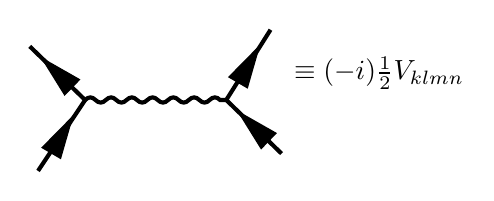
\begin{tikzpicture}[x=0.75pt,y=0.75pt,yscale=-1,xscale=1]
%uncomment if require: \path (0,705); %set diagram left start at 0, and has height of 705
%Straight Lines [id:da613823184290475] 
\draw [line width=1.5]    (436.42,562.13) .. controls (438.09,560.46) and (439.75,560.46) .. (441.42,562.13) .. controls (443.09,563.8) and (444.75,563.8) .. (446.42,562.13) .. controls (448.09,560.46) and (449.75,560.46) .. (451.42,562.13) .. controls (453.09,563.8) and (454.75,563.8) .. (456.42,562.13) .. controls (458.09,560.46) and (459.75,560.46) .. (461.42,562.13) .. controls (463.09,563.8) and (464.75,563.8) .. (466.42,562.13) .. controls (468.09,560.46) and (469.75,560.46) .. (471.42,562.13) .. controls (473.09,563.8) and (474.75,563.8) .. (476.42,562.13) .. controls (478.09,560.46) and (479.75,560.46) .. (481.42,562.13) .. controls (483.09,563.8) and (484.75,563.8) .. (486.42,562.13) .. controls (488.09,560.46) and (489.75,560.46) .. (491.42,562.13) .. controls (493.09,563.8) and (494.75,563.8) .. (496.42,562.13) .. controls (498.09,560.46) and (499.75,560.46) .. (501.42,562.13) -- (504.42,562.13) -- (504.42,562.13) ;
%Straight Lines [id:da6353755682299548] 
\draw [line width=1.5]    (409.75,536.3) -- (436.42,562.13) ;
%Straight Lines [id:da6254606220772768] 
\draw [line width=1.5]    (504.42,562.13) -- (531.08,587.97) ;
%Straight Lines [id:da5480869883300985] 
\draw [line width=1.5]    (436.42,562.13) -- (413.75,596.3) ;
%Straight Lines [id:da49445752084181116] 
\draw [line width=1.5]    (525.75,528.3) -- (504.42,562.13) ;
%Shape: Triangle [id:dp022384072825595847] 
\draw  [fill={rgb, 255:red, 0; green, 0; blue, 0 }  ,fill opacity=1 ] (416.18,542.57) -- (433.37,552.35) -- (426.61,559.37) -- cycle ;
%Shape: Triangle [id:dp5669679661948073] 
\draw  [fill={rgb, 255:red, 0; green, 0; blue, 0 }  ,fill opacity=1 ] (510.84,568.41) -- (528.04,578.18) -- (521.28,585.21) -- cycle ;
%Shape: Triangle [id:dp23872151900315752] 
\draw  [fill={rgb, 255:red, 0; green, 0; blue, 0 }  ,fill opacity=1 ] (519.92,536.94) -- (514.46,555.95) -- (506.04,551.03) -- cycle ;
%Shape: Triangle [id:dp5504301680867448] 
\draw  [fill={rgb, 255:red, 0; green, 0; blue, 0 }  ,fill opacity=1 ] (429.92,570.94) -- (424.46,589.95) -- (416.04,585.03) -- cycle ;

% Text Node
\draw (535.68,539.7) node [anchor=north west][inner sep=0.75pt]    {$\equiv ( -i)\frac{1}{2} V_{klmn}$};
\end{tikzpicture}
\end{center}
Using the particle-hole formalism, this may be drawn in more detail, thus:
\begin{equation}
    \includegraphics[width=0.8\textwidth]{screenshots/wiggly-diagram-types.PNG}
    \label{wiggly-types}
\end{equation}
Diagram (a) pictures scattering of two particles at state $\phi_m$ and $\phi_n$ into $\phi_k$ and $\phi_l$. In (b) a particle at state $\phi_m$ interacts with another particle below the Fermi surface in state $\phi_n$ to create a hole in $\phi_n$ and a particle in $\phi_l$. At the same time the original particle undergoes a transition to state $\phi_k$. Note that the diagrams in \ref{wiggly-types} correspond precisely to the interaction terms in the Hamiltonian of \ref{mutual-interact-hamiltonian}.
\begin{imp}
It is extremely important to note the labelling convention used in $V_{k l m n}: \mathbf{k}=$ line out of left vertex, $\mathbf{l}=$ line out of right vertex, $\mathbf{m}=$ line into left vertex, $\mathbf{n}=$ line into right vertex. A mnemonic aid is to remember the tango dance step: \textbf{left out, right out, left in, right in.}
\end{imp}
\redp{The interaction $V(|\mathbf{r}-\mathbf{r}^{\prime}|)$ only depends on the distance between the particles so it conserves linear and spin momentum.} Thus
$$\mathbf{k}+\mathbf{l}=\mathbf{m}+\mathbf{n} ; \quad \boldsymbol{\sigma}_{k}+\boldsymbol{\sigma}_{l}=\boldsymbol{\sigma}_{m}+\boldsymbol{\sigma}_{n}$$
We can incorporate this conservation law into our diagrams by labelling the "momentum flow" shown below:
\begin{equation}
\tikzset{every picture/.style={line width=0.75pt}} %set default line width to 0.75pt        
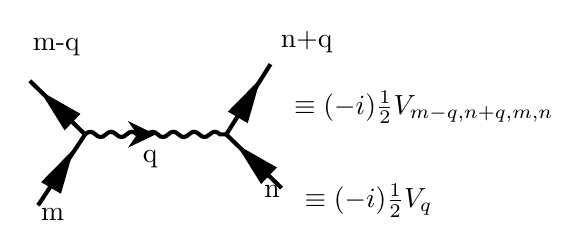
\begin{tikzpicture}[x=0.75pt,y=0.75pt,yscale=-1,xscale=1]
%uncomment if require: \path (0,705); %set diagram left start at 0, and has height of 705
%Straight Lines [id:da613823184290475] 
\draw [line width=1.5]    (416.42,563.13) .. controls (418.09,561.46) and (419.75,561.46) .. (421.42,563.13) .. controls (423.09,564.8) and (424.75,564.8) .. (426.42,563.13) .. controls (428.09,561.46) and (429.75,561.46) .. (431.42,563.13) .. controls (433.09,564.8) and (434.75,564.8) .. (436.42,563.13) .. controls (438.09,561.46) and (439.75,561.46) .. (441.42,563.13) .. controls (443.09,564.8) and (444.75,564.8) .. (446.42,563.13) .. controls (448.09,561.46) and (449.75,561.46) .. (451.42,563.13) .. controls (453.09,564.8) and (454.75,564.8) .. (456.42,563.13) .. controls (458.09,561.46) and (459.75,561.46) .. (461.42,563.13) .. controls (463.09,564.8) and (464.75,564.8) .. (466.42,563.13) .. controls (468.09,561.46) and (469.75,561.46) .. (471.42,563.13) .. controls (473.09,564.8) and (474.75,564.8) .. (476.42,563.13) .. controls (478.09,561.46) and (479.75,561.46) .. (481.42,563.13) -- (484.42,563.13) -- (484.42,563.13) ;
\draw [shift={(450.42,563.13)}, rotate = 180] [fill={rgb, 255:red, 0; green, 0; blue, 0 }  ][line width=0.08]  [draw opacity=0] (13.4,-6.43) -- (0,0) -- (13.4,6.44) -- (8.9,0) -- cycle    ;
%Straight Lines [id:da6353755682299548] 
\draw [line width=1.5]    (389.75,537.3) -- (416.42,563.13) ;
%Straight Lines [id:da6254606220772768] 
\draw [line width=1.5]    (484.42,563.13) -- (511.08,588.97) ;
%Straight Lines [id:da5480869883300985] 
\draw [line width=1.5]    (416.42,563.13) -- (393.75,597.3) ;
%Straight Lines [id:da49445752084181116] 
\draw [line width=1.5]    (505.75,529.3) -- (484.42,563.13) ;
%Shape: Triangle [id:dp022384072825595847] 
\draw  [fill={rgb, 255:red, 0; green, 0; blue, 0 }  ,fill opacity=1 ] (396.18,543.57) -- (413.37,553.35) -- (406.61,560.37) -- cycle ;
%Shape: Triangle [id:dp5669679661948073] 
\draw  [fill={rgb, 255:red, 0; green, 0; blue, 0 }  ,fill opacity=1 ] (490.84,569.41) -- (508.04,579.18) -- (501.28,586.21) -- cycle ;
%Shape: Triangle [id:dp23872151900315752] 
\draw  [fill={rgb, 255:red, 0; green, 0; blue, 0 }  ,fill opacity=1 ] (499.92,537.94) -- (494.46,556.95) -- (486.04,552.03) -- cycle ;
%Shape: Triangle [id:dp5504301680867448] 
\draw  [fill={rgb, 255:red, 0; green, 0; blue, 0 }  ,fill opacity=1 ] (409.92,571.94) -- (404.46,590.95) -- (396.04,586.03) -- cycle ;

% Text Node
\draw (515.68,540.7) node [anchor=north west][inner sep=0.75pt]    {$\equiv ( -i)\frac{1}{2} V_{m-q,n+q,m,n}$};
% Text Node
\draw (393.75,597.3) node [anchor=north west][inner sep=0.75pt]   [align=left] {m};
% Text Node
\draw (389.75,515.3) node [anchor=north west][inner sep=0.75pt]   [align=left] {m-q};
% Text Node
\draw (442.75,569.3) node [anchor=north west][inner sep=0.75pt]   [align=left] {q};
% Text Node
\draw (501.28,586.21) node [anchor=north west][inner sep=0.75pt]   [align=left] {n};
% Text Node
\draw (509.28,512.21) node [anchor=north west][inner sep=0.75pt]   [align=left] {n+q};
% Text Node
\draw (520.68,585.7) node [anchor=north west][inner sep=0.75pt]    {$\equiv ( -i)\frac{1}{2} V_{q}$};


\end{tikzpicture}
\label{momentum-flow}
\end{equation}
By changing the dummy indices in \ref{Vklmn-defi} we have $V_{klmn}=V_{lknm}$, so $V_q=V_{-q}$. $V_{-q}$ corresponds to the diagram in \ref{momentum-flow} twisted through $180^o$, has momentum transfer $\mathbf{q}^{\prime}=\mathbf{n}-\mathbf{l}$.
\begin{imp}
It is important to note that although the collisions conserves momentum, they do not conserve energy. For example, at the lower interaction of the diagram shown below we see the energy flow into the interaction \bluep{(in the unit of $\hbar^2/2m$)} is $k^2+l^2$, while the energy flow out is $(k-q)^2+(l+q)^2$. Hence we are dealing with virtual particles during the interactions.
\begin{center}
    


\tikzset{every picture/.style={line width=0.75pt}} %set default line width to 0.75pt        

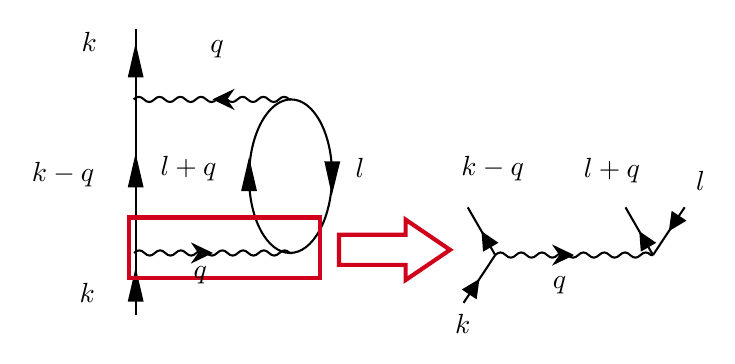
\begin{tikzpicture}[x=0.75pt,y=0.75pt,yscale=-1,xscale=1]
%uncomment if require: \path (0,244); %set diagram left start at 0, and has height of 244

%Straight Lines [id:da8265491360075683] 
\draw    (62.53,30.8) -- (62.53,168.8) ;
%Straight Lines [id:da7214893814207295] 
\draw    (61.53,64.8) .. controls (63.2,63.13) and (64.86,63.13) .. (66.53,64.8) .. controls (68.2,66.47) and (69.86,66.47) .. (71.53,64.8) .. controls (73.2,63.13) and (74.86,63.13) .. (76.53,64.8) .. controls (78.2,66.47) and (79.86,66.47) .. (81.53,64.8) .. controls (83.2,63.13) and (84.86,63.13) .. (86.53,64.8) .. controls (88.2,66.47) and (89.86,66.47) .. (91.53,64.8) .. controls (93.2,63.13) and (94.86,63.13) .. (96.53,64.8) .. controls (98.2,66.47) and (99.86,66.47) .. (101.53,64.8) .. controls (103.2,63.13) and (104.86,63.13) .. (106.53,64.8) .. controls (108.2,66.47) and (109.86,66.47) .. (111.53,64.8) .. controls (113.2,63.13) and (114.86,63.13) .. (116.53,64.8) .. controls (118.2,66.47) and (119.86,66.47) .. (121.53,64.8) .. controls (123.2,63.13) and (124.86,63.13) .. (126.53,64.8) .. controls (128.2,66.47) and (129.86,66.47) .. (131.53,64.8) .. controls (133.2,63.13) and (134.86,63.13) .. (136.53,64.8) -- (137.53,64.8) -- (137.53,64.8) ;
\draw [shift={(99.53,64.8)}, rotate = 0] [fill={rgb, 255:red, 0; green, 0; blue, 0 }  ][line width=0.08]  [draw opacity=0] (10.72,-5.15) -- (0,0) -- (10.72,5.15) -- (7.12,0) -- cycle    ;
%Straight Lines [id:da6531867980247327] 
\draw    (61.78,138.78) .. controls (63.45,137.11) and (65.11,137.11) .. (66.78,138.78) .. controls (68.45,140.45) and (70.11,140.45) .. (71.78,138.78) .. controls (73.45,137.11) and (75.11,137.11) .. (76.78,138.78) .. controls (78.45,140.45) and (80.11,140.45) .. (81.78,138.78) .. controls (83.45,137.11) and (85.11,137.11) .. (86.78,138.78) .. controls (88.45,140.45) and (90.11,140.45) .. (91.78,138.78) .. controls (93.45,137.11) and (95.11,137.11) .. (96.78,138.78) .. controls (98.45,140.45) and (100.11,140.45) .. (101.78,138.78) .. controls (103.45,137.11) and (105.11,137.11) .. (106.78,138.78) .. controls (108.45,140.45) and (110.11,140.45) .. (111.78,138.78) .. controls (113.45,137.11) and (115.11,137.11) .. (116.78,138.78) .. controls (118.45,140.45) and (120.11,140.45) .. (121.78,138.78) .. controls (123.45,137.11) and (125.11,137.11) .. (126.78,138.78) .. controls (128.45,140.45) and (130.11,140.45) .. (131.78,138.78) .. controls (133.45,137.11) and (135.11,137.11) .. (136.78,138.78) -- (137.78,138.78) -- (137.78,138.78) ;
\draw [shift={(99.78,138.78)}, rotate = 180] [fill={rgb, 255:red, 0; green, 0; blue, 0 }  ][line width=0.08]  [draw opacity=0] (10.72,-5.15) -- (0,0) -- (10.72,5.15) -- (7.12,0) -- cycle    ;
%Shape: Ellipse [id:dp27679763462197615] 
\draw   (136.78,138.78) .. controls (125.74,138.67) and (116.95,122.02) .. (117.16,101.59) .. controls (117.37,81.16) and (126.49,64.69) .. (137.53,64.8) .. controls (148.58,64.91) and (157.36,81.56) .. (157.16,101.99) .. controls (156.95,122.42) and (147.83,138.89) .. (136.78,138.78) -- cycle ;
%Shape: Triangle [id:dp5635326143074989] 
\draw  [fill={rgb, 255:red, 0; green, 0; blue, 0 }  ,fill opacity=1 ] (117.16,94.73) -- (120.35,108.45) -- (113.97,108.45) -- cycle ;
%Shape: Triangle [id:dp24603935178928227] 
\draw  [fill={rgb, 255:red, 0; green, 0; blue, 0 }  ,fill opacity=1 ] (157.07,108.86) -- (154.06,95.09) -- (160.44,95.17) -- cycle ;
%Shape: Triangle [id:dp6426129992054267] 
\draw  [fill={rgb, 255:red, 0; green, 0; blue, 0 }  ,fill opacity=1 ] (62.53,92.94) -- (65.72,106.66) -- (59.35,106.66) -- cycle ;
%Shape: Triangle [id:dp6567192777691618] 
\draw  [fill={rgb, 255:red, 0; green, 0; blue, 0 }  ,fill opacity=1 ] (62.53,39.94) -- (65.72,53.66) -- (59.35,53.66) -- cycle ;
%Shape: Triangle [id:dp3743764640683508] 
\draw  [fill={rgb, 255:red, 0; green, 0; blue, 0 }  ,fill opacity=1 ] (62.53,147.94) -- (65.72,161.66) -- (59.35,161.66) -- cycle ;
%Shape: Rectangle [id:dp8012947756470761] 
\draw  [color={rgb, 255:red, 208; green, 2; blue, 27 }  ,draw opacity=1 ][line width=1.5]  (59.35,121.66) -- (151.53,121.66) -- (151.53,150.8) -- (59.35,150.8) -- cycle ;
%Right Arrow [id:dp412985882083701] 
\draw  [color={rgb, 255:red, 208; green, 2; blue, 27 }  ,draw opacity=1 ][line width=1.5]  (160.53,130) -- (192.61,130) -- (192.61,122.73) -- (214,137.27) -- (192.61,151.8) -- (192.61,144.53) -- (160.53,144.53) -- cycle ;
%Straight Lines [id:da9760212638037913] 
\draw    (235.78,139.78) .. controls (237.45,138.11) and (239.11,138.11) .. (240.78,139.78) .. controls (242.45,141.45) and (244.11,141.45) .. (245.78,139.78) .. controls (247.45,138.11) and (249.11,138.11) .. (250.78,139.78) .. controls (252.45,141.45) and (254.11,141.45) .. (255.78,139.78) .. controls (257.45,138.11) and (259.11,138.11) .. (260.78,139.78) .. controls (262.45,141.45) and (264.11,141.45) .. (265.78,139.78) .. controls (267.45,138.11) and (269.11,138.11) .. (270.78,139.78) .. controls (272.45,141.45) and (274.11,141.45) .. (275.78,139.78) .. controls (277.45,138.11) and (279.11,138.11) .. (280.78,139.78) .. controls (282.45,141.45) and (284.11,141.45) .. (285.78,139.78) .. controls (287.45,138.11) and (289.11,138.11) .. (290.78,139.78) .. controls (292.45,141.45) and (294.11,141.45) .. (295.78,139.78) .. controls (297.45,138.11) and (299.11,138.11) .. (300.78,139.78) .. controls (302.45,141.45) and (304.11,141.45) .. (305.78,139.78) .. controls (307.45,138.11) and (309.11,138.11) .. (310.78,139.78) -- (311.78,139.78) -- (311.78,139.78) ;
\draw [shift={(273.78,139.78)}, rotate = 180] [fill={rgb, 255:red, 0; green, 0; blue, 0 }  ][line width=0.08]  [draw opacity=0] (10.72,-5.15) -- (0,0) -- (10.72,5.15) -- (7.12,0) -- cycle    ;
%Straight Lines [id:da4571267837545099] 
\draw    (222.53,116.8) -- (235.78,139.78) ;
\draw [shift={(229.16,128.29)}, rotate = 60.03] [fill={rgb, 255:red, 0; green, 0; blue, 0 }  ][line width=0.08]  [draw opacity=0] (8.93,-4.29) -- (0,0) -- (8.93,4.29) -- cycle    ;
%Straight Lines [id:da08135471840003439] 
\draw    (235.78,139.78) -- (220.53,162.8) ;
\draw [shift={(228.16,151.29)}, rotate = 123.53] [fill={rgb, 255:red, 0; green, 0; blue, 0 }  ][line width=0.08]  [draw opacity=0] (8.93,-4.29) -- (0,0) -- (8.93,4.29) -- cycle    ;
%Straight Lines [id:da42744127070386173] 
\draw    (327.04,116.76) -- (311.78,139.78) ;
\draw [shift={(319.41,128.27)}, rotate = 303.53] [fill={rgb, 255:red, 0; green, 0; blue, 0 }  ][line width=0.08]  [draw opacity=0] (8.93,-4.29) -- (0,0) -- (8.93,4.29) -- cycle    ;
%Straight Lines [id:da3731869684683673] 
\draw    (298.53,116.8) -- (311.78,139.78) ;
\draw [shift={(305.16,128.29)}, rotate = 60.03] [fill={rgb, 255:red, 0; green, 0; blue, 0 }  ][line width=0.08]  [draw opacity=0] (8.93,-4.29) -- (0,0) -- (8.93,4.29) -- cycle    ;

% Text Node
\draw (11,93.73) node [anchor=north west][inner sep=0.75pt]    {$k-q$};
% Text Node
\draw (35,30.73) node [anchor=north west][inner sep=0.75pt]    {$k$};
% Text Node
\draw (34,151.73) node [anchor=north west][inner sep=0.75pt]    {$k$};
% Text Node
\draw (73,90.73) node [anchor=north west][inner sep=0.75pt]    {$l+q$};
% Text Node
\draw (167,91.73) node [anchor=north west][inner sep=0.75pt]    {$l$};
% Text Node
\draw (97,34.73) node [anchor=north west][inner sep=0.75pt]    {$q$};
% Text Node
\draw (89,143.73) node [anchor=north west][inner sep=0.75pt]    {$q$};
% Text Node
\draw (218,90.73) node [anchor=north west][inner sep=0.75pt]    {$k-q$};
% Text Node
\draw (215,166.73) node [anchor=north west][inner sep=0.75pt]    {$k$};
% Text Node
\draw (262,148.73) node [anchor=north west][inner sep=0.75pt]    {$q$};
% Text Node
\draw (331,97.73) node [anchor=north west][inner sep=0.75pt]    {$l$};
% Text Node
\draw (277,91.73) node [anchor=north west][inner sep=0.75pt]    {$l+q$};


\end{tikzpicture}
\end{center}
\end{imp}
The diagram in the box above depicts a particle in $\mathbf{k}$ being scattered into $\mathbf{k}-\mathbf{q}$ and simultaneously knocking a particle out of $\mathbf{l}$ into $\mathbf{l}+\mathbf{q}$ (i.e., creating a particle in $\mathbf{l}+\mathbf{q}$ and a hole in $\mathbf{l}$. At later time, the particle in $\mathbf{k}-\mathbf{q}$ knocks the particle in $\mathbf{l}+\mathbf{q}$ back into the hole state $\mathbf{l}$ (thus annihilating the particle-hole pair) and is itself scattered into state $\mathbf{k}$. \textbf{This is a second-order process, because it involves two interactions.}

The possibilities of first-order interactions are shown below
\begin{equation}
    \includegraphics[width=0.8\textwidth]{screenshots/first-order-wiggly.PNG}
\end{equation}
The diagrams such as
\begin{center}
\tikzset{every picture/.style={line width=0.75pt}} %set default line width to 0.75pt        

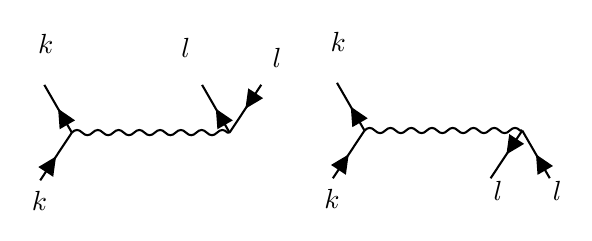
\begin{tikzpicture}[x=0.75pt,y=0.75pt,yscale=-1,xscale=1]
%uncomment if require: \path (0,244); %set diagram left start at 0, and has height of 244

%Straight Lines [id:da9760212638037913] 
\draw    (93.78,111.78) .. controls (95.45,110.11) and (97.11,110.11) .. (98.78,111.78) .. controls (100.45,113.45) and (102.11,113.45) .. (103.78,111.78) .. controls (105.45,110.11) and (107.11,110.11) .. (108.78,111.78) .. controls (110.45,113.45) and (112.11,113.45) .. (113.78,111.78) .. controls (115.45,110.11) and (117.11,110.11) .. (118.78,111.78) .. controls (120.45,113.45) and (122.11,113.45) .. (123.78,111.78) .. controls (125.45,110.11) and (127.11,110.11) .. (128.78,111.78) .. controls (130.45,113.45) and (132.11,113.45) .. (133.78,111.78) .. controls (135.45,110.11) and (137.11,110.11) .. (138.78,111.78) .. controls (140.45,113.45) and (142.11,113.45) .. (143.78,111.78) .. controls (145.45,110.11) and (147.11,110.11) .. (148.78,111.78) .. controls (150.45,113.45) and (152.11,113.45) .. (153.78,111.78) .. controls (155.45,110.11) and (157.11,110.11) .. (158.78,111.78) .. controls (160.45,113.45) and (162.11,113.45) .. (163.78,111.78) .. controls (165.45,110.11) and (167.11,110.11) .. (168.78,111.78) -- (169.78,111.78) -- (169.78,111.78) ;
%Straight Lines [id:da4571267837545099] 
\draw    (80.53,88.8) -- (93.78,111.78) ;
\draw [shift={(87.16,100.29)}, rotate = 60.03] [fill={rgb, 255:red, 0; green, 0; blue, 0 }  ][line width=0.08]  [draw opacity=0] (8.93,-4.29) -- (0,0) -- (8.93,4.29) -- cycle    ;
%Straight Lines [id:da08135471840003439] 
\draw    (93.78,111.78) -- (78.53,134.8) ;
\draw [shift={(86.16,123.29)}, rotate = 123.53] [fill={rgb, 255:red, 0; green, 0; blue, 0 }  ][line width=0.08]  [draw opacity=0] (8.93,-4.29) -- (0,0) -- (8.93,4.29) -- cycle    ;
%Straight Lines [id:da42744127070386173] 
\draw    (185.04,88.76) -- (169.78,111.78) ;
\draw [shift={(177.41,100.27)}, rotate = 303.53] [fill={rgb, 255:red, 0; green, 0; blue, 0 }  ][line width=0.08]  [draw opacity=0] (8.93,-4.29) -- (0,0) -- (8.93,4.29) -- cycle    ;
%Straight Lines [id:da3731869684683673] 
\draw    (156.53,88.8) -- (169.78,111.78) ;
\draw [shift={(163.16,100.29)}, rotate = 60.03] [fill={rgb, 255:red, 0; green, 0; blue, 0 }  ][line width=0.08]  [draw opacity=0] (8.93,-4.29) -- (0,0) -- (8.93,4.29) -- cycle    ;
%Straight Lines [id:da9023180120241947] 
\draw    (234.78,110.78) .. controls (236.45,109.11) and (238.11,109.11) .. (239.78,110.78) .. controls (241.45,112.45) and (243.11,112.45) .. (244.78,110.78) .. controls (246.45,109.11) and (248.11,109.11) .. (249.78,110.78) .. controls (251.45,112.45) and (253.11,112.45) .. (254.78,110.78) .. controls (256.45,109.11) and (258.11,109.11) .. (259.78,110.78) .. controls (261.45,112.45) and (263.11,112.45) .. (264.78,110.78) .. controls (266.45,109.11) and (268.11,109.11) .. (269.78,110.78) .. controls (271.45,112.45) and (273.11,112.45) .. (274.78,110.78) .. controls (276.45,109.11) and (278.11,109.11) .. (279.78,110.78) .. controls (281.45,112.45) and (283.11,112.45) .. (284.78,110.78) .. controls (286.45,109.11) and (288.11,109.11) .. (289.78,110.78) .. controls (291.45,112.45) and (293.11,112.45) .. (294.78,110.78) .. controls (296.45,109.11) and (298.11,109.11) .. (299.78,110.78) .. controls (301.45,112.45) and (303.11,112.45) .. (304.78,110.78) .. controls (306.45,109.11) and (308.11,109.11) .. (309.78,110.78) -- (310.78,110.78) -- (310.78,110.78) ;
%Straight Lines [id:da768308410681679] 
\draw    (221.53,87.8) -- (234.78,110.78) ;
\draw [shift={(228.16,99.29)}, rotate = 60.03] [fill={rgb, 255:red, 0; green, 0; blue, 0 }  ][line width=0.08]  [draw opacity=0] (8.93,-4.29) -- (0,0) -- (8.93,4.29) -- cycle    ;
%Straight Lines [id:da7130025901944149] 
\draw    (234.78,110.78) -- (219.53,133.8) ;
\draw [shift={(227.16,122.29)}, rotate = 123.53] [fill={rgb, 255:red, 0; green, 0; blue, 0 }  ][line width=0.08]  [draw opacity=0] (8.93,-4.29) -- (0,0) -- (8.93,4.29) -- cycle    ;
%Straight Lines [id:da8657016622612258] 
\draw    (310.78,110.78) -- (295.53,133.8) ;
\draw [shift={(303.16,122.29)}, rotate = 303.53] [fill={rgb, 255:red, 0; green, 0; blue, 0 }  ][line width=0.08]  [draw opacity=0] (8.93,-4.29) -- (0,0) -- (8.93,4.29) -- cycle    ;
%Straight Lines [id:da9413606756365827] 
\draw    (310.78,110.78) -- (324.04,133.76) ;
\draw [shift={(317.41,122.27)}, rotate = 60.03] [fill={rgb, 255:red, 0; green, 0; blue, 0 }  ][line width=0.08]  [draw opacity=0] (8.93,-4.29) -- (0,0) -- (8.93,4.29) -- cycle    ;

% Text Node
\draw (76,62.73) node [anchor=north west][inner sep=0.75pt]    {$k$};
% Text Node
\draw (73,138.73) node [anchor=north west][inner sep=0.75pt]    {$k$};
% Text Node
\draw (189,69.73) node [anchor=north west][inner sep=0.75pt]    {$l$};
% Text Node
\draw (145,64.73) node [anchor=north west][inner sep=0.75pt]    {$l$};
% Text Node
\draw (217,61.73) node [anchor=north west][inner sep=0.75pt]    {$k$};
% Text Node
\draw (214,137.73) node [anchor=north west][inner sep=0.75pt]    {$k$};
% Text Node
\draw (324.04,133.76) node [anchor=north west][inner sep=0.75pt]    {$l$};
% Text Node
\draw (295.53,133.8) node [anchor=north west][inner sep=0.75pt]    {$l$};


\end{tikzpicture}
\end{center}
are \bluep{not allowed since they have a particle and a hole in the same state $\mathbf{l}$.} It can be shown that diagrams (1),(3),(5) and (7) above do not occur either. The term in disturbed Hamiltonian that corresponds to (1) is 
\begin{equation}
    V_{klkl}a^{\dagger}_ka^{\dagger}_la_ka_l
\end{equation}
when this acts on the state with one incoming particle in $\phi_k$, we find
$$V_{k l k l} a_{k}^{\dagger} a_{l}^{\dagger} a_{k} a_{l}|1^p_k\rangle=0$$
Diagrams (3),(5), and (7) are similarly eliminated. Note that the term in $H_1$ corresponding to diagram (2) is (following the rule of left-out,right-out, left-in,right-in):
\begin{equation}V_{k l k l} a_{k}^{\dagger}b_l a_{k} b_{l}^{\dagger}\end{equation}
and
\begin{equation}V_{k l k l}  a_{k}^{\dagger}b_{l} a_{k} b_{l}^{\dagger}\left|1_{k}^{p}\right\rangle=V_{k l k l}\left|1_{k}^{p}\right\rangle \neq 0\end{equation}
The possible first-order processes may then be drawn using (2),(4),(6),(8). \textbf{This can only be done in one way, e.g., by in each case attaching the outgoing $\mathbf{l}$ line to the incoming one. Thus we find:}
\begin{equation}
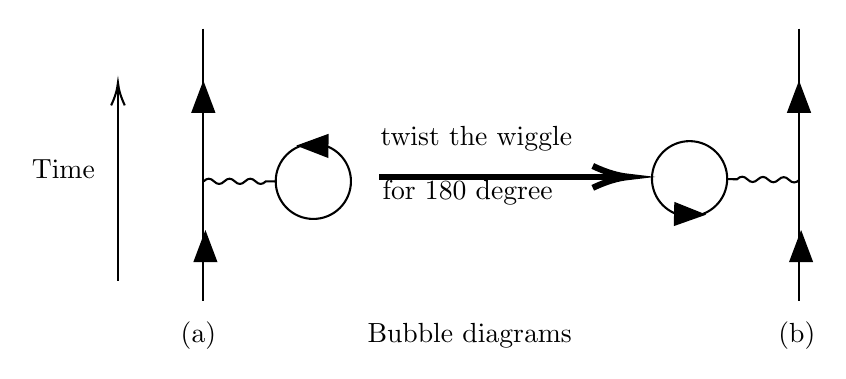
\begin{tikzpicture}[x=0.75pt,y=0.75pt,yscale=-1,xscale=1]
%uncomment if require: \path (0,235); %set diagram left start at 0, and has height of 235

%Straight Lines [id:da10068577398388545] 
\draw    (172,46.6) -- (172,178) ;
%Shape: Triangle [id:dp19925235312138345] 
\draw  [fill={rgb, 255:red, 0; green, 0; blue, 0 }  ,fill opacity=1 ] (172.13,73) -- (177.25,86.6) -- (167,86.6) -- cycle ;
%Shape: Triangle [id:dp004394430560968221] 
\draw  [fill={rgb, 255:red, 0; green, 0; blue, 0 }  ,fill opacity=1 ] (173.13,145) -- (178.25,158.6) -- (168,158.6) -- cycle ;
%Shape: Circle [id:dp41514745661808317] 
\draw   (207,120.13) .. controls (207,110.11) and (215.11,102) .. (225.13,102) .. controls (235.14,102) and (243.25,110.11) .. (243.25,120.13) .. controls (243.25,130.14) and (235.14,138.25) .. (225.13,138.25) .. controls (215.11,138.25) and (207,130.14) .. (207,120.13) -- cycle ;
%Straight Lines [id:da9922958867186198] 
\draw    (172.25,120.13) .. controls (173.92,118.46) and (175.58,118.46) .. (177.25,120.13) .. controls (178.92,121.8) and (180.58,121.8) .. (182.25,120.13) .. controls (183.92,118.46) and (185.58,118.46) .. (187.25,120.13) .. controls (188.92,121.8) and (190.58,121.8) .. (192.25,120.13) .. controls (193.92,118.46) and (195.58,118.46) .. (197.25,120.13) .. controls (198.92,121.8) and (200.58,121.8) .. (202.25,120.13) -- (207,120.13) -- (207,120.13) ;
%Shape: Triangle [id:dp2263151698703949] 
\draw  [fill={rgb, 255:red, 0; green, 0; blue, 0 }  ,fill opacity=1 ] (218.33,102.93) -- (231.98,97.95) -- (231.87,108.19) -- cycle ;
%Straight Lines [id:da3409503459639508] 
\draw    (459,46.6) -- (459,178) ;
%Shape: Triangle [id:dp7202483298889484] 
\draw  [fill={rgb, 255:red, 0; green, 0; blue, 0 }  ,fill opacity=1 ] (459.13,73) -- (464.25,86.6) -- (454,86.6) -- cycle ;
%Shape: Triangle [id:dp05921608545174617] 
\draw  [fill={rgb, 255:red, 0; green, 0; blue, 0 }  ,fill opacity=1 ] (460.13,145) -- (465.25,158.6) -- (455,158.6) -- cycle ;
%Shape: Circle [id:dp43994714997441664] 
\draw   (424.52,119.08) .. controls (424.42,129.09) and (416.22,137.12) .. (406.21,137.01) .. controls (396.2,136.91) and (388.17,128.71) .. (388.27,118.7) .. controls (388.38,108.69) and (396.58,100.66) .. (406.59,100.76) .. controls (416.6,100.87) and (424.63,109.07) .. (424.52,119.08) -- cycle ;
%Straight Lines [id:da8513266846637301] 
\draw    (459.27,119.44) .. controls (457.58,121.09) and (455.92,121.08) .. (454.27,119.39) .. controls (452.62,117.71) and (450.95,117.69) .. (449.27,119.34) .. controls (447.59,120.99) and (445.92,120.97) .. (444.27,119.29) .. controls (442.62,117.6) and (440.96,117.58) .. (439.27,119.23) .. controls (437.59,120.88) and (435.92,120.86) .. (434.27,119.18) .. controls (432.62,117.5) and (430.95,117.48) .. (429.27,119.13) -- (424.52,119.08) -- (424.52,119.08) ;
%Shape: Triangle [id:dp20595976463490984] 
\draw  [fill={rgb, 255:red, 0; green, 0; blue, 0 }  ,fill opacity=1 ] (413.02,136.15) -- (399.31,141) -- (399.53,130.75) -- cycle ;
%Straight Lines [id:da9038937323503633] 
\draw [line width=2.25]    (257,118) -- (373.25,118) ;
\draw [shift={(377.25,118)}, rotate = 180] [color={rgb, 255:red, 0; green, 0; blue, 0 }  ][line width=2.25]    (17.49,-5.26) .. controls (11.12,-2.23) and (5.29,-0.48) .. (0,0) .. controls (5.29,0.48) and (11.12,2.23) .. (17.49,5.26)   ;
%Straight Lines [id:da5407884786763255] 
\draw    (131,168) -- (131,74.6) ;
\draw [shift={(131,72.6)}, rotate = 450] [color={rgb, 255:red, 0; green, 0; blue, 0 }  ][line width=0.75]    (10.93,-3.29) .. controls (6.95,-1.4) and (3.31,-0.3) .. (0,0) .. controls (3.31,0.3) and (6.95,1.4) .. (10.93,3.29)   ;

% Text Node
\draw (256,92) node [anchor=north west][inner sep=0.75pt]   [align=left] {twist the wiggle};
% Text Node
\draw (257,118) node [anchor=north west][inner sep=0.75pt]   [align=left] {for 180 degree};
% Text Node
\draw (88,108) node [anchor=north west][inner sep=0.75pt]   [align=left] {Time};
% Text Node
\draw (159.73,186.07) node [anchor=north west][inner sep=0.75pt]   [align=left] {(a)};
% Text Node
\draw (447.73,186.07) node [anchor=north west][inner sep=0.75pt]   [align=left] {(b)};
% Text Node
\draw (249.73,187.07) node [anchor=north west][inner sep=0.75pt]   [align=left] {Bubble diagrams};


\end{tikzpicture}
\label{bubble-diagrams}
\end{equation}
\begin{equation}
    \includegraphics[width=0.8\textwidth]{screenshots/open-oyster-diagrams.PNG}
    \label{open-oyster-diagrams}
\end{equation}
The bubble processes can be physically interpreted as follows: a particle enters in $\mathbf{k}>k_F$, knocks a particle out of state $\mathbf{l}<k_F$ at time t, then knocks the particle instantaneously back into $\mathbf{l}$ at time t, then continues freely in state $\mathbf{k}$.

The open-oyster processes are just like the bubbles, except that a quick change act occurs in which at time $t$ the incoming particle simultaneously
(a) strikes the particle in $\mathbf{l},(b)$ creates an instantaneous hole in $\mathbf{l}$ and $(c)$ is exchanged for the particle in $\mathbf{l}.$ Diagrams \ref{open-oyster-diagrams}) are often called "first-order exchange diagrams', and the process is referred to as an \textbf{"exchange scattering"}. The instantaneous hole lines in the bubble and open oyster are called \textbf{"non-propagating"} lines.

We now see how to evaluate these diagrams. Consider \ref{bubble-diagrams}(a), we have
\begin{equation}\begin{array}{l}
G^+(\mathbf{k},t_2-t_1)=(-1) \sum_{l<k_{F}} \int_{-\infty}^{+\infty} d t\left[i G_{0}^{+}\left(\mathbf{k}, t-t_{1}\right)\right] \times\left[-\frac{i}{2} V_{k l k l}\right] \times \\
\quad \times\left[i G_{0}^{-}(l, t-t)\right] \times\left[i G_{0}^{+}\left(\mathbf{k}, t_{2}-t\right)\right]
\end{array}\end{equation}
\redp{The extra factor of (-1) in front comes from the fact that the diagram contains one \textbf{"fermion loop"}.} Note that an additional factor of (-1) appears because the propagator line for the bubble is:
\begin{equation}i G_{0}^{-}(1, t-t)=i \times i e^{-i\epsilon_l \times 0}=-1\end{equation}
The Fourier transform is then
\begin{equation}
G^+(\mathbf{k},\omega)=(-1)\left[i G_{0}^{+}(\mathbf{k}, \omega)\right]^{2} \sum_{i<k_{r}}\left[-\frac{i}{2} V_{k l k l}\right](-1)\end{equation}
In a similar fashion, \ref{bubble-diagrams}(b) is
\begin{equation}(-1)\left[i G^+(\mathbf{k},\omega)=G_{0}(\mathbf{k}, \omega)\right]^{2} \sum_{l<k_{r}}\left(-\frac{i}{2}\right) V_{l k l k}(-1)\end{equation}
Since $V_{klkl}=V_{lklk}$ these diagrams are equivalent. From here, we have the following rule:
\begin{imp}
If we are given a diagram, and form a new diagram from it by twisting one or more of its interaction wiggles through 180 degrees, then the new diagram has the same value as the original one. Hence all twisted diagrams may be omitted if we just multiply a correct factor in front.
\end{imp}
In a manner similar to the bubble diagram calculation, the open oyser gives
\begin{equation}
    G^+(\mathbf{k},\omega)=[iG^+_0(\mathbf{k},\omega)]^2\sum_{l<k_F}(-i)V_{lkkl}(-1)
\end{equation}
where the factor of 2 is included, and (-1) comes from $G^{-}_0(\mathbf{k},t-t)$. Observe that the frequency, $\omega$, associated with the propagator line coming out of the interaction is the same as that entering. This is an illustration of "\textbf{conservation of frequency}", and it is a result from the fact that \redp{the Hamiltonian is time-dependent.}

We now summarize the dictionary for the expansion series
\begin{figure}
    \centering
    \includegraphics[width=0.8\textwidth]{screenshots/interacting-fermi-sys-dict.PNG}
    \caption{Diagram dictionary for interacting many-fermion system with no external potential (Goldstone method)}
    \label{fig:goldstone-interacting-fermi-dict}
\end{figure}
The diagrams may also be interpreted physically from a particular time $t_0$:
\begin{center}
    \includegraphics[width=0.8\textwidth]{screenshots/goldstone-particular-time.PNG}
\end{center}
At $t_{0}$ we see that besides the bare particle, there may exist in the many-body system two "virtual' particles plus one hole created by second-order process $d$ or two particles and a hole created by second-order sequence $e,$ and so on, with the particle plus three particle-hole pairs created during the eighth-order poodle process illustrating a typical higher-order case. That is, \textbf{the diagrams show all the particles and holes which may be kicked up by the bare particle as it churns through the Fermi sea.}
\subsection{The "quasi-physical" nature of Feynman diagrams}